\documentclass{beamer}

\usepackage[ngerman]{babel}
\usepackage[utf8]{inputenc}
\usepackage{hyperref}

\mode<presentation>{
	\definecolor{LogoRed}{RGB}{219,00,31}
	\definecolor{LogoGray}{RGB}{86,86,80}
	
	\useoutertheme[width=2.1cm]{sidebar}
	\useinnertheme{rounded}
	\setbeamercolor{normal text}{fg=black,bg=white}
	\setbeamercolor{palette sidebar primary}{use=normal text,fg=normal text.fg}
	\setbeamercolor{title}{fg=LogoRed}
	\setbeamercolor{frametitle}{fg=LogoRed}
	\setbeamercolor{structure}{fg=LogoRed}
	\setbeamercolor{section in sidebar}{fg=LogoRed}
	\setbeamercolor{subsection in sidebar}{fg=LogoRed}
	
	\usefoottemplate{\vbox{\tinycolouredline{LogoGray!25}{\hspace{4pt}\hspace{15pt}\insertdate\hfill\insertshortinstitute\hfill \insertframenumber{}/\inserttotalframenumber}}}
	
	\setbeamertemplate{section in toc}{\inserttocsectionnumber.~\inserttocsection\par}
	\setbeamertemplate{subsection in toc}{\hspace*{2em}\inserttocsectionnumber.\inserttocsubsectionnumber~\inserttocsubsection}
	\AtBeginSubsection[] {
		\begin{frame}<beamer>
			\frametitle{Outline}
			\tableofcontents[currentsection,sectionstyle=show/show,subsectionstyle=show/shaded/hide]
		\end{frame}
	}
}

\title{Vorkurs WS 2015/16}
\author[Diana Irmscher]{Diana Irmscher\\\texttt{irmscher@fs.cs.hm.edu}}
\institute[Fachschaft 07]{Fachschaft 07\\Fakultät für Informatik und Mathematik\\Hochschule für angewandte Wissenschaften München}
\logo{
\includegraphics[height=1.5cm]{logo_fs07.pdf}}
\date{\today}

\setbeamertemplate{navigation symbols}{}

\begin{document}
	\maketitle
	
	\section{Begrüßung}
	
	\begin{frame}
		\frametitle{Organisation}
		\begin{columns}[t]
			\column{.47\textwidth}
			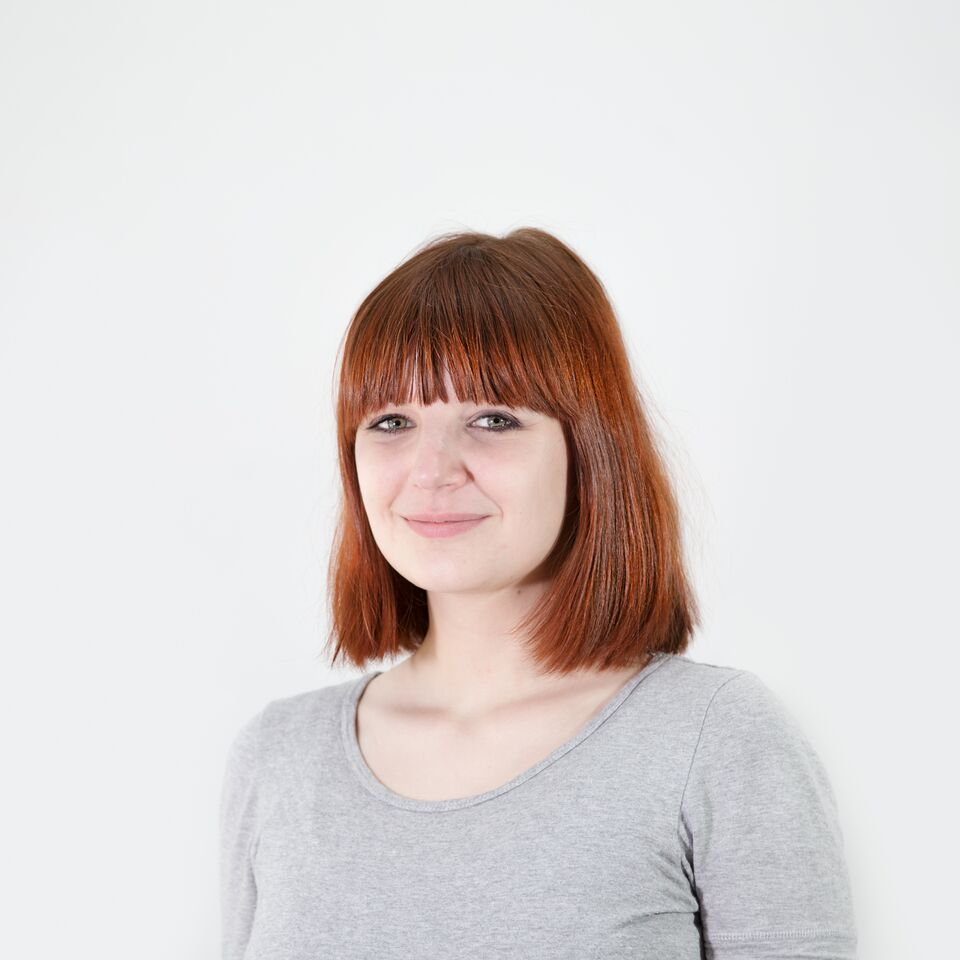
\includegraphics[width=0.5\textwidth]{diana.jpg}
			\\Diana Irmscher
			\column{.47\textwidth}
			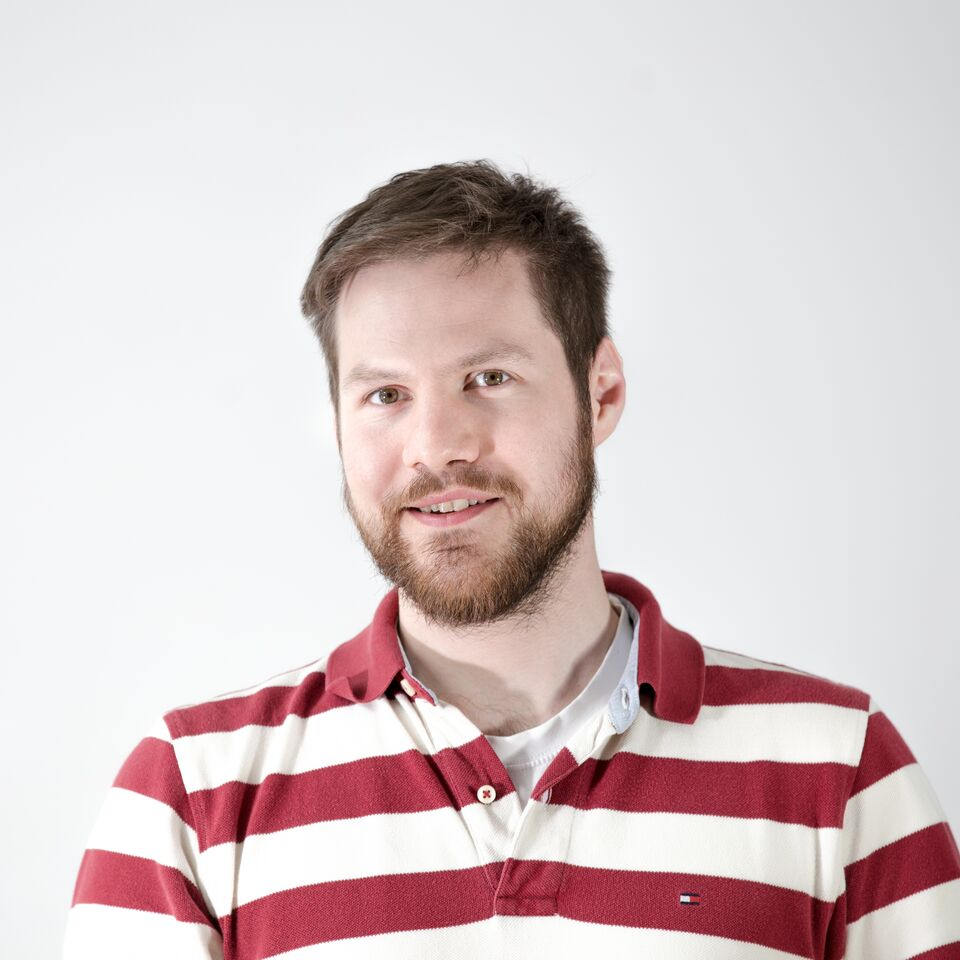
\includegraphics[width=0.5\textwidth]{ersin.jpg}
			\\Ersin Öztürk
		\end{columns}
		\bigskip
		\bigskip
		Helfer
		\begin{itemize}
			\item Nicole Behrens
			\item Sebastian Klohn
		\end{itemize}
	\end{frame}
	
	\begin{frame}
		\begin{columns}[t]
			\column{.47\textwidth}
			\frametitle{Dozenten}
			Mathematik
			\begin{itemize}
				\item Chris Becker
				\item Benedikt Zönnchen
				\item Sebastian Klohn
				\item Lesya Mankovska
				\item Felix Dietrich
				\item Marc Zibelink
				\item Linda Rudolph
				\item Stephan Plöderl
			\end{itemize}
			\column{.47\textwidth}
			Softwareentwicklung
			\begin{itemize}
				\item Fabio Hellmann
				\item Benjamin Klas
				\item Tim Lauster
				\item Luca Spataro
				\item Christian Worf
				\item Benjamin Reischböck
				\item Daniela Zehetmeier
			\end{itemize}
		\end{columns}
	\end{frame}
	
	\begin{frame}
		\frametitle{Agenda}
		\tableofcontents
	\end{frame}
	
	\section{Termine}
	\begin{frame}
		\frametitle{Termine}
		Erstsemesterveranstaltung
		\begin{itemize}
			\item Donnerstag, 01.10.2015 um 09:00 Uhr im Roten Würfel
		\end{itemize}
		\pause
		Erstsemestertag der Fakultät
		\begin{itemize}
			\item Freitag, 02.10.2015 ab 08:15 Uhr in der Lothstraße 64
		\end{itemize}
		\pause
		Wahl der AW-Fächer
		\begin{itemize}
			\item 17.09. - 02.10.2015: Belegung 1. Los-Durchgang
			\item 05.10.2015: Bekanntgabe des 1. Los-Durchgangs
			\item 05.10. - 06.10.2015: Belegung 2. Los-Durchgang
			\item 07.10.2015: Bekanntgabe des 2. Los-Durchgangs
		\end{itemize}
	\end{frame}
	
	\section{Die Fachschaft}
	
	\begin{frame}[t]
		\frametitle{Fachschaftsleitung}
		\center
		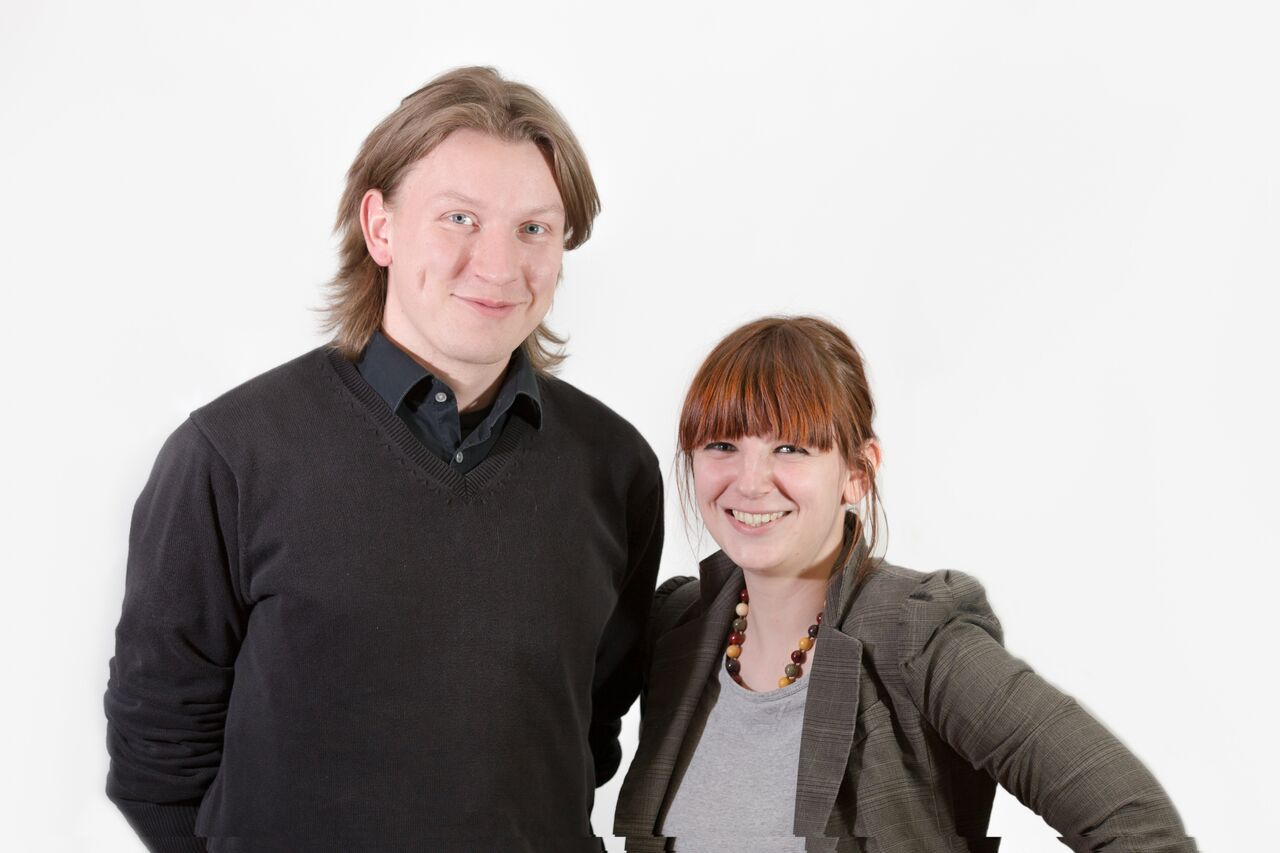
\includegraphics[width=0.7\textwidth]{matti_diana.jpg}
		\\Mathias Duve und Diana Irmscher
	\end{frame}
	
	\begin{frame}[t]
		\frametitle{... aber wir sind noch viel mehr}
		\center
		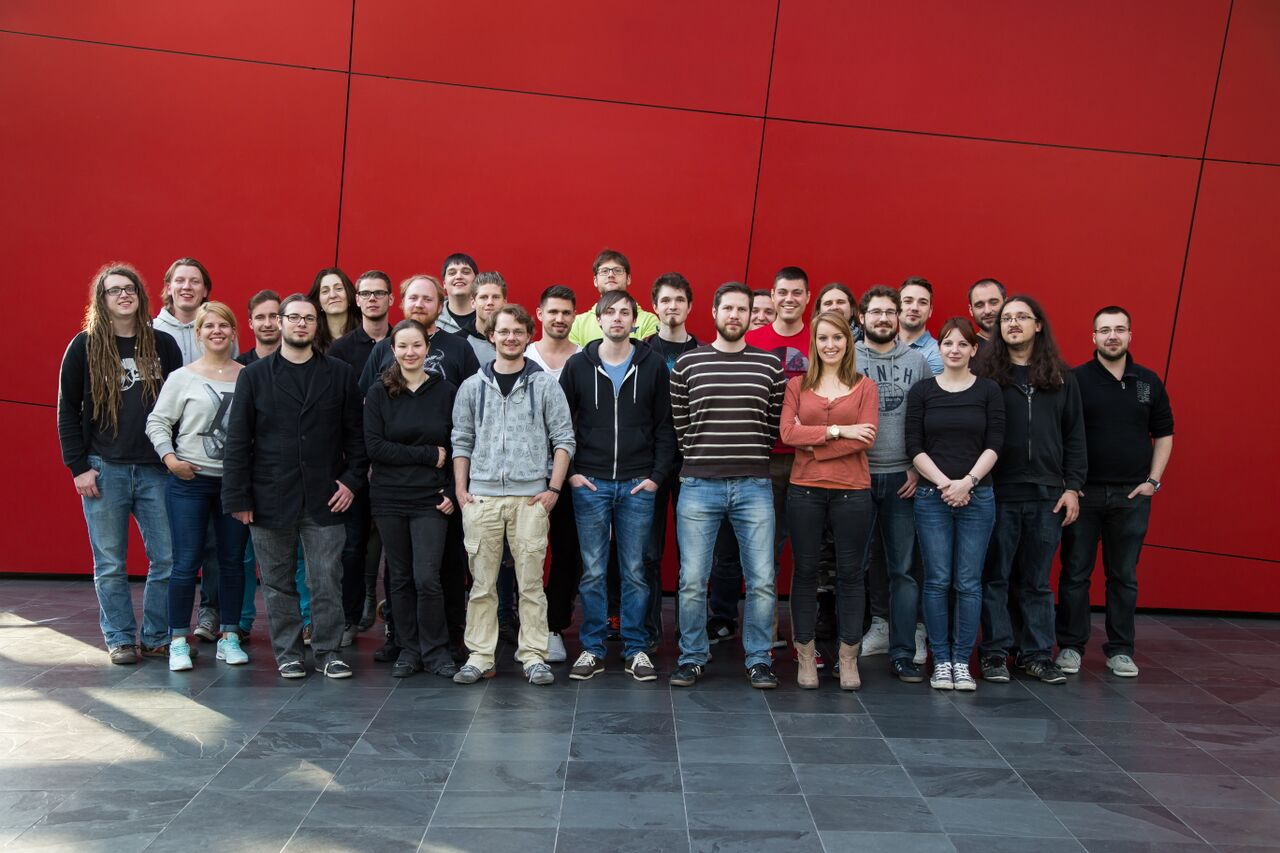
\includegraphics[width=1\textwidth]{fachschaft.jpg}
		\\Fachschaft im letzten Semester
	\end{frame}
	
	\begin{frame}[t]
		\frametitle{Was macht die Fachschaft?}
		
		\begin{itemize}
			\item Ansprechpartner für Fragen zum Studium
			\item Rechts- und Studienberatung
			\item Fakultätsrat
			\item Paritätische Kommission
			\item Studentisches Parlament
			\item Social Media
		\end{itemize}
		\bigskip
		\begin{itemize}
			\item Vorkurs
			\item Erstsemesterveranstaltung
			\item Studentische Vollversammlung
			\item RetroGaming Abend
			\item Speeddating (Firmenkontakte)
			\item Absolventenfeier
		\end{itemize}
	\end{frame}
	
	\begin{frame}[t]
		\frametitle{ErstiGuide}
		Wir haben wichtige Informationen für Erstsemester in einem Guide für euch zusammengestellt.\\
		\bigskip
		Download unter \url{fs.cs.hm.edu}\\
		\center
		
\includegraphics[width=0.3\textwidth]{erstiguide.jpg}
	\end{frame}
	
	\section{Studium}
	
	\begin{frame}[t]
		\frametitle{Accounts}
		\begin{itemize}
			\item Hochschul-Account
			\begin{itemize}
				\item Mail-Postfach unter \url{xmail.mwn.de}
			\end{itemize}
			\pause
			\item Moodle (E-Learning-Plattform)
			\begin{itemize}
				\item Mail-Postfach unter \url{moodle.hm.edu}
			\end{itemize}
			\pause
			\item Eduroam (WLAN)
			\begin{itemize}
				\item \url{www.lrz.de/services/netz/mobil/wireless/}
			\end{itemize}
			\pause
			\item LRZ (VPN/WLAN)
			\begin{itemize}
				\item \url{www.lrz.de/services/netz/mobil/vpn/}
			\end{itemize}
		\end{itemize}
	\end{frame}
	
	\begin{frame}[t]
		\frametitle{Accounts}
		\begin{itemize}
			\item FK07-Kennung
			\begin{itemize}
				\item ifw-Account, z.B. ifw12345
				\item Laborrechner
			\end{itemize}
			\pause
			\item ZPA-System
			\begin{itemize}
				\item \url{w3-o.cs.hm.edu/zpa/}
				\item Anmeldung mit FK07-Account
				\item Anmeldung für FWP-Fächer (mit und ohne Praktika),
				praxisbegleitenden Unterricht,
				Blockunterricht,
				Praktika zu bestimmten Vorlesungen und
				Seminaren
			\end{itemize}
		\end{itemize}
	\end{frame}
	
	\begin{frame}
		\frametitle{Veranstaltungen}
		Anwesenheitspflicht in Vorlesungen?
		\begin{itemize}
			\item in den meisten Veranstaltungen nicht, in Seminaren (z.B. Angewandte Mathematik) jedoch schon
			\item dennoch ratsam, gerade am Beginn des Studium jede Veranstaltung zu besuchen
		\end{itemize}
		\bigskip
		\pause
		Zwischen den Vorlesungen
		\begin{itemize}
			\item Lernen, Essen, Entspannen
			\item Aufenthaltsräume
		\end{itemize}
		\bigskip
		\pause
		Nach den Vorlesungen
		\begin{itemize}
			\item Lernen
			\item Abgaben vorbereiten
		\end{itemize}
		
	\end{frame}
	
	\begin{frame}[t]
		\frametitle{Tipps für's Studium}
		\begin{itemize}
			\item Lerngruppen
			\pause
			\item Wahl des Praktikumspartners
			\pause
			\item Organisation des Studiums: Prüfungen schieben ist immer schlecht
			\pause
			\item eigenes Notebook ist empfehlenswert
			\pause
			\item Bücher bekommt man alle in der Bibliothek \url{bib.hm.edu}
		\end{itemize}
	\end{frame}
	
	\begin{frame}[t]
		\frametitle{Tipps für's Studium}
		\begin{itemize}
			\item Unterlagen, Skripte 
			\begin{itemize}
				\item Moodle
				\item Skriptensammlung der Fachschaft
				\item Skriptenbestellung der Fachschaft
			\end{itemize}
			\pause
			\item Website der Fachschaft\\ \url{fs.cs.hm.edu}
			\pause
			\item Android-App der Fachschaft\\ \url{play.google.com/store/apps/details?id=com.fk07}
			\pause
			\item iOS-App der Fachschaft\\
			in Arbeit	
		\end{itemize}
	\end{frame}
	
	\section{Vorkurs}
	
	\begin{frame}
		\frametitle{Themen im Vorkurs}
		Softwareentwicklung
		\begin{itemize}
			\item Grundkenntnisse der Programmierung mit Java
			\item Seminar
		\end{itemize}
		\bigskip
		Mathematik
		\begin{itemize}
			\item Themen aus der Analysis
			\item Vorlesung und Übung
		\end{itemize}
	\end{frame}
	
	\begin{frame}
		\frametitle{Stundenplan}
		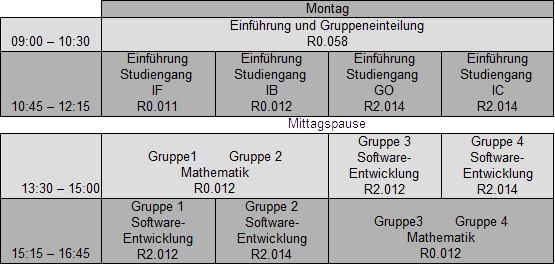
\includegraphics[width=1\textwidth]{montag.png}
	\end{frame}
	
	\begin{frame}
		\frametitle{Stundenplan}
		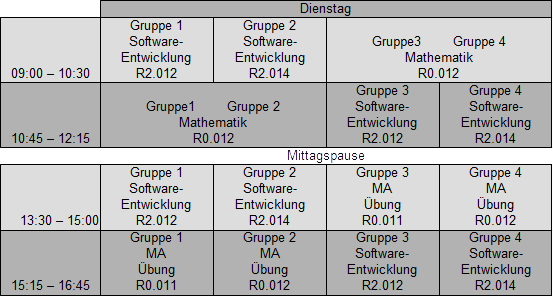
\includegraphics[width=1\textwidth]{dienstag.png}
	\end{frame}
	
	\begin{frame}
		\frametitle{Stundenplan}
		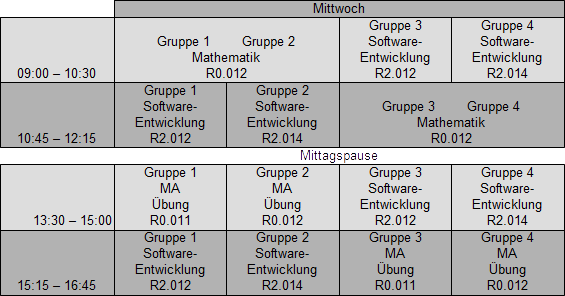
\includegraphics[width=1\textwidth]{mittwoch.png}
	\end{frame}
	
	\begin{frame}
		\frametitle{Stundenplan}
		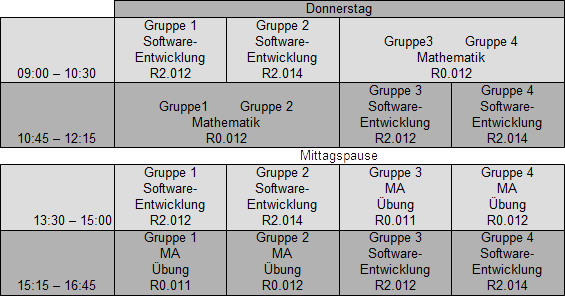
\includegraphics[width=1\textwidth]{donnerstag.png}
	\end{frame}
	
	\begin{frame}
		\frametitle{Stundenplan}
		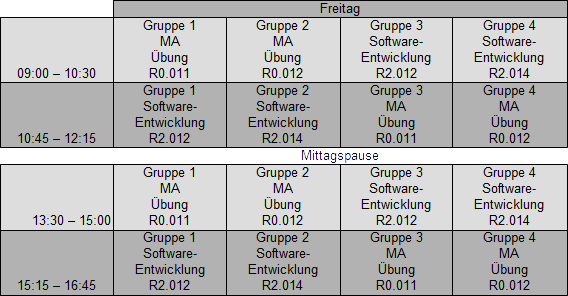
\includegraphics[width=1\textwidth]{freitag.png}
	\end{frame}
	
	\begin{frame}
		\frametitle{Themen im Vorkurs}
		Gruppeneinteilung
	\end{frame}
	
	\begin{frame}
		\center Danke für eure Aufmerksamkeit\\ und\\ viel Spaß beim Vorkurs!
	\end{frame}

\end{document}